\section{Desenvolvimento da Rede Neural Artificial}

Para realizar a determinação das intensidades de chuvas por meio de redes neurais artificiais, utilizou-se um microcomputador com processador Intel Core i7 @ 2.95 GHz e 16 GB de RAM, operando sob a plataforma Microsoft Windows 10. A linguagem de programação escolhida foi o Matlab.

O desenvolvimento de um projeto baseado em RNA envolve diversas etapas como mostra a Figura \ref{fig:fluxograma}. 

\begin{figure}[h]
    \caption{Diagrama do sistema para determinação da intensidade de chuva}
    \centering
    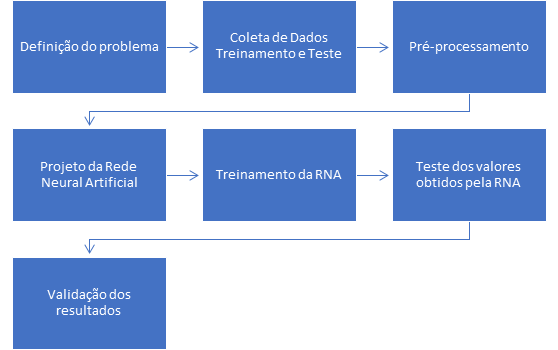
\includegraphics[width=0.70\textwidth]{Textuais/Figuras/fluxograma.png}
    \fonte{Autores}
    \label{fig:fluxograma}
\end{figure}

\subsection{Definição do problema}

Conforme descrito no capítulo 3, uma rede neural artificial de aproximação tem como funcionalidade determinar os pesos $w_i$, obtendo-se uma equação que melhor se ajusta aos dados de saída.

A ideia proposta é a utilização do Teorema Universal de Aproximação para conseguir representar as relações de intensidade-duração-frequência da região Recife.

\subsection{Coleta de dados}

%explicar sobre a série: que série?
O registro pluviográfico utilizado nesse trabalho foi fornecido pelo Instituto de Tecnologia de Pernambuco (ITEP). Após análise dos dados, foram descartadas as séries em que houve falha nos registros das precipitações. Para o ajuste da RNA foram considerados os dados entre 2003 e 2011.

\subsection{Projeto da RNA}

Os sistemas baseados em RNA dependem vigorosamente da topologia dessas redes, da mesma maneira que os parâmetros de entrada. Como resposta, a determinação da arquitetura está correlacionada com o seu desempenho, isto é, está relacionada com a precisão e velocidade de processamento do aprendizado. Devido à qualidade e quantidade de dados disponíveis existe uma grande dificuldade em desenvolver uma rede neural com uma grande capacidade de generalização.

\subsection{Treinamento da RNA}

Os pesos sinápticos presentes nas redes neurais artificiais são responsáveis pelo conhecimento adquirido pela rede. São esses parâmetros que deverão ser ajustados em um processo denominado “treinamento”, tornando possível a rede responder o melhor possível a quaisquer outros valores que lhe forem apresentados, em uma fase posterior, chamada de teste.

Em uma primeira etapa, é apresentada para a rede uma fração dos dados para treinamento. Esse conjunto de dados contém informações suficientes para a rede conseguir inferir relações entre os dados. Esse treinamento segue uma metodologia: o conjunto de dados, sem respostas, é inserido na rede. A rede irá gerar uma resposta que é comparada com a resposta dos dados de teste e os pesos são ajustados. Esse processo é repetido inúmeras vezes, até que a rede consiga acertar as respostas ou quando o erro seja minimizado. 

\subsection{Teste dos resultados obtidos}

Após o treinamento da rede neural, é apresentado à rede um novo conjunto de dados, com as mesmas características, porém diferentes, dos dados apresentados durante a fase de treinamento. 

\subsection{Validação dos resultados}

Com a finalidade de validar a rede neural, serão calculados três erros: o Erro Total, Erro Médio e Erro Máximo. O Erro Total é o somatório da diferença entre o resultado da rede e o resultado esperado. O Erro Médio é dado pelo Erro Total dividido pela quantidade de dados. E o Erro Máximo é a maior diferença entre o valor esperado e o valor determinado pela rede.

